\documentclass{uimppracticas}

%Permitir cabeceras y pie de páginas personalizados
\pagestyle{fancy}

%Path por defecto de las imágenes
\graphicspath{ {./images/} }

%Declarar formato de encabezado y pie de página de las páginas del documento
\fancypagestyle{doc}{
  %Pie de Página
  \footerpr{}{}{{\thepage} de \pageref{LastPage}}
}

%Declarar formato de encabezado y pie del título e indice
\fancypagestyle{titu}{%
  %Cabecera
  \headerpr{}{}{}
  %Pie de Página
  \footerpr{}{}{}
}

\appto\frontmatter{\pagestyle{titu}}
\appto\mainmatter{\pagestyle{doc}}

\begin{document}
	
%Comienzo formato título
\frontmatter

%Portada (Centrado todo)
\centeredtitle{./images/LogoUIMP.png}{Máster Universitario en Investigación en Inteligencia Artificial}{Curso 2020-2021}{Recuperación y extracción de información, \\ grafos y redes sociales}{Práctica Bloque II: Recuperación de información y minería de texto}

\begin{center}
\large \today
\end{center}

\vspace{40mm}

\begin{flushright}
 	{\bf Laura Rodríguez Navas}\\
 	\textbf{DNI:} 43630508Z\\
 	\textbf{e-mail:} \href{rodrigueznavas@posgrado.uimp.es}{rodrigueznavas@posgrado.uimp.es}
\end{flushright}

\newpage

%Índice
\tableofcontents

\newpage

%Comienzo formato documento general
\mainmatter

\setlength\parskip{2.5ex}

\section{Resumen}

En esta práctica se ha implementado un rastreador web (crawler) en Python~\cite{GitHubRepo} (ver Sección~\ref{crawler}), que se complementa con un proceso de agrupamiento (ver Sección~\ref{kmeans}), también implementado en Python, de la información extraída por el rastreador web. 

\section{Rastreador web (crawler)}\label{crawler}

En esta sección se describe como se ha implementado el rastreador web (crawler) en Python usando la librería \href{https://scrapy.org/}{Scrapy}. Para empezar con la implementación se debe ejecutar el siguiente comando:

\begin{lstlisting}[language=bash]
$ scrapy startproject books
\end{lstlisting}

Este comando crea un proyecto Scrapy en el directorio books, siguiendo la \href{https://docs.scrapy.org/en/latest/topics/commands.html#default-structure-of-scrapy-projects}{estructura por defecto}, común para todo proyecto Scrapy. También crea el fichero \textit{scrapy.cfg}, que contiene el nombre del módulo en Python que define la configuración del proyecto books (\textit{books.settings}). El proyecto lo he nombrado books, porqué se rastreará y se recuperará información de un catálogo de libros que se encuentra en la página web: \url{http://books.toscrape.com}.

Una vez se ha creado el proyecto, se tienen que definir los ítems de cada libro que se quieran extraer del catálogo. En este caso los ítems que se van a extraer son: el título, la categoría, la descripción, el precio y la valoración de cada libro. Para ello, se tiene que modificar el fichero \textit{books/items.py}, para incluir los cinco ítems que se quieren extraer. Vemos el contenido de \textit{items.py} a continuación:

\begin{lstlisting}[language=python]
import scrapy

class BooksItem(scrapy.Item):
	# define the fields for your item here like:
	# name = scrapy.Field()
	title = scrapy.Field()
	category = scrapy.Field()
	description = scrapy.Field()
	price = scrapy.Field()
	rating = scrapy.Field()
\end{lstlisting}

El siguiente paso es describir la manera de extraer la información definida en el fichero \textit{items.py}. Para ello, se utilizan reglas de expresión \href{https://www.w3.org/TR/xpath/all/}{XPath} y \href{https://www.w3.org/TR/selectors/}{CSS}. Por ejemplo, si nos fijamos en el código HTML de uno de los libros que se van rastrear (ver Figura \ref{book}), veremos que el título del libro es fácil de extraer con la siguiente regla de expresión CSS: \textbf{"h1 ::text"}. Pero cuando la extracción de información se complica un poco más, se usan reglas de expresión XPath. Por ejemplo, para extraer las descripciones de todos los libros se usará la regla de expresión: \textbf{"//div[@id='product\_description']/following-sibling::p/text()"}. Una vez, definidas todas las reglas de expresión para cada ítem que se va a rastrear, se crea la araña \textit{books/spiders/books\_toscrape.py}.

\begin{figure}[h]
	\centering
	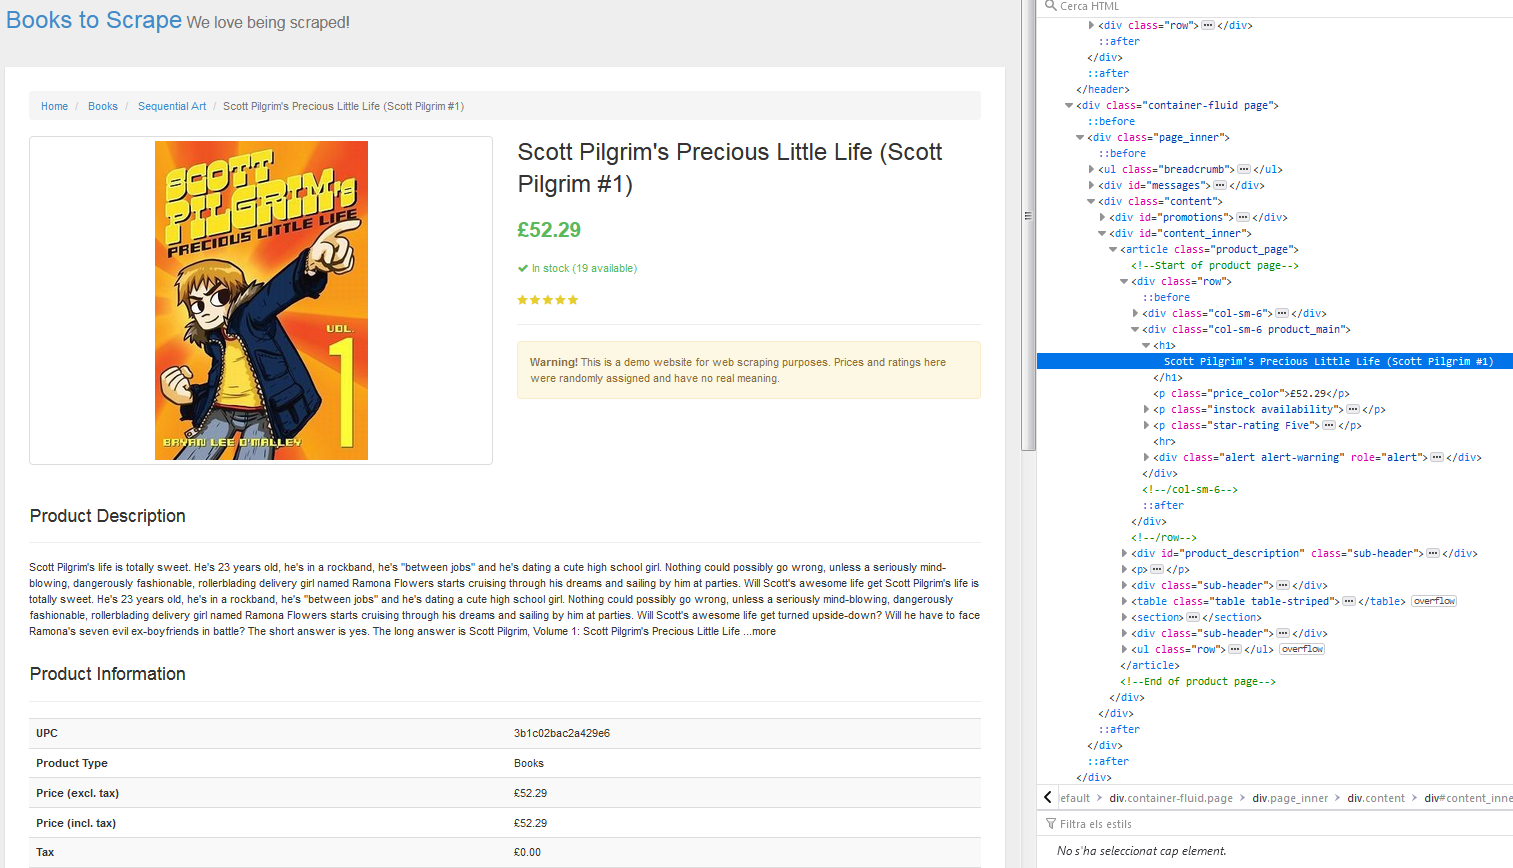
\includegraphics[scale=0.33]{images/book}
	\caption{Ejemplo de libro a rastrear.}
	\label{book}
\end{figure}

\begin{definition}\label{spider}
Las arañas son clases que definen cómo se rastrea una página web determinada (o un grupo de páginas web), incluido cómo realizar el rastreo y cómo extraer la información deseada. En otras palabras, las arañas son el lugar donde se define el comportamiento personalizado para rastrear y analizar las páginas web.
\end{definition}

En el caso de la práctica, la araña \textit{books.toscrape} representará el lugar donde se definen las reglas de expresión. En las arañas también se tienen que especificar las solicitudes iniciales para rastrear las URLs y una función de devolución de llamada (\textit{parse}) a la que se llamará para generar los ítems de respuesta de esas solicitudes. Por último, los ítems devueltos por las arañas normalmente se conservan en una base de datos o se escriben en un archivo. En el caso de la práctica, los ítems (título, categoría, descripción, precio y valoración de cada libro) devueltos por la araña serán guardados en el fichero \textit{books.json}. La araña \textit{books.toscrape} que procesa todas las URLs descubiertas de \url{http://books.toscrape.com}, utilizando la función \textit{parse} que a su vez llama a la función \textit{parse\_book\_page} donde son definidas todas las reglas de expresión de cómo extraer la información deseada, se muestra a continuación:

\begin{lstlisting}[language=python]
import scrapy

class BooksToscrapeSpider(scrapy.Spider):
	name = 'books.toscrape'
	allowed_domains = ['books.toscrape.com']
	start_urls = ['http://books.toscrape.com/']
	
	def parse(self, response):
		for book_url in response.css("article.product_pod > h3 > a ::attr(href)").extract():
			yield scrapy.Request(response.urljoin(book_url), callback=self.parse_book_page)
		next_page = response.css("li.next > a ::attr(href)").extract_first()
		if next_page:
			yield scrapy.Request(response.urljoin(next_page), callback=self.parse)
	
	@staticmethod
	def parse_book_page(response):
		item = {}
		product = response.css("div.product_main")
		item["title"] = product.css("h1 ::text").extract_first()
		item['category'] = response.xpath("//ul[@class='breadcrumb']/li[@class='active']/preceding-sibling::li[1]/a/text()").extract_first()
		item['description'] = response.xpath("//div[@id='product_description']/following-sibling::p/text()").extract_first()
		price = response.xpath('//th[text()="Price (incl. tax)"]/following-sibling::td/text()').extract_first()
		item['price'] = price.replace('£', '')
		rating = response.xpath('//*[contains(@class, "star-rating")]/@class').extract_first()
		item['rating'] = rating.replace('star-rating ', '')
		yield item
\end{lstlisting}

En este momento ya podemos iniciar la araña para que recupere la información del catálogo web y la guarde en el fichero \textit{books.json}, aunque primero es recomendable modificar el fichero \textit{books/settings.py} para limitar el acceso de la araña al catálogo web, ya que podemos generar un ataque \href{https://es.wikipedia.org/wiki/Ataque_de_denegaci%C3%B3n_de_servicio}{DDoS}. Para ello, debemos descomentar la variable \href{https://docs.scrapy.org/en/latest/topics/settings.html#download-delay}{DOWNLOAD\_DELAY} y darle un valor en segundos (p.ej. DOWNLOAD\_DELAY = 3). 
	
Para iniciar la araña se debe ejecutar el siguiente comando:	
	
\begin{lstlisting}[language=bash]
	$ cd books
	$ scrapy crawl books.toscrape -o books.json
\end{lstlisting}

\section{K-Means}\label{kmeans} 

En esta sección se describe como se ha implementado el proceso de agrupamiento en Python, usando la librería scikit-learn~\cite{scikit-learn}. La implementación llevada a cabo se encuentra en el directorio kmeans en~\cite{GitHubRepo}. Concretamente, el algoritmo de agrupación elegido para esta práctica ha sido:  \href{https://scikit-learn.org/stable/modules/generated/sklearn.cluster.KMeans.html}{K-Means}. En el caso de la práctica, el algoritmo K-Means agrupará los títulos de los libros del catálogo web, recuperados en la Sección~\ref{crawler}, en diferentes clústeres.

\subsection{Datos de entrada}

Si nos fijamos en la implementación del fichero \textit{kmeans/kmeans.py}, concretamente en el \textit{main}, vemos que empezamos extrayendo la información de los libros del catálogo web, almacenada en el fichero \textit{books/books.json}, y la convertimos en un \textit{DataFrame} (ver Definición~\ref{dataframe}). A continuación, se eliminan los valores NaN que pudieran existir en \textit{DataFrame} y este es almacenado en un fichero CSV (\textit{kmeans/books.csv}). Para este proceso se usa la librería pandas~\cite{jeff_reback_2020_4309786}.

Las primeras líneas del \textit{DataFrame} que forman los datos de entrada:

\begin{table}[h]
	\begin{adjustbox}{width=\columnwidth,center}
		\begin{tabular}{lllll}
			\toprule
			title & category & description & price & rating \\
			\midrule
			Sapiens: A Brief History of Humankind & History & From a renowned historian... & 54.23 & Five \\
			Sharp Objects & Mystery & WICKED above her hipbone, GIRL... & 47.82 & Four \\
			Soumission & Fiction & Dans une France assez... & 50.10 & One \\
			Tipping the Velvet & Historical Fiction & Erotic and absorbing... & 53.74 & One \\
			A Light in the Attic & Poetry & It's hard to imagine... & 51.77 & Three \\
			\bottomrule
		\end{tabular}
	\end{adjustbox}
	\caption{Conjunto de datos de entrada.}
	\label{table1}
\end{table}

Llegados a este punto, se concreta la estructura de datos que se utilizará para alimentar el algoritmo K-Means. Se crea una lista que contiene los títulos de los libros.

\begin{lstlisting}[language=python]
titles = df["title"].to_list()
print(titles[:10])  # first 10 titles
>> ['Sapiens: A Brief History of Humankind', 'Sharp Objects', 'Soumission', 'Tipping the Velvet', 'A Light in the Attic', "It's Only the Himalayas", 'Libertarianism for Beginners', 'Mesaerion: The Best Science Fiction Stories 1800-1849', 'Olio', 'Our Band Could Be Your Life: Scenes from the American Indie Underground, 1981-1991']
\end{lstlisting}

\begin{definition}\label{dataframe}
Un DataFrame es una estructura de datos bidimensional etiquetada que acepta diferentes tipos datos de entrada organizados en columnas. Se puede pensar en un DataFrame como una hoja de cálculo o una tabla SQL.
\end{definition}

\subsection{Palabras vacías, stemming y tokenización}\label{stem_token}

Esta sección se centra en definir algunas funciones para transformar el texto de los títulos de los libros para facilitar el entrenamiento del algoritmo K-Means. Para empezar, se obtiene la lista de palabras vacías en inglés (ver Definición~\ref{palabras_vacías}), utilizando la librería NLTK~\cite{bird2009natural}. La lista de palabras vacías es en inglés ya que los títulos de los libros están inglés. Después, se obtiene el \textit{Snowball Stemmer}, también utilizando la librería NLTK, para descomponer las palabras que forman cada título en sus raíces correspondientes.

\begin{lstlisting}[language=python]
# nltk's English stopwords as variable called 'stopwords'	
stopwords = nltk.corpus.stopwords.words('english')  
# nltk's SnowballStemmer as variabled 'stemmer'
stemmer = SnowballStemmer("english")
print(stopwords[:10])   # first 10 stopwords
>> ['i', 'me', 'my', 'myself', 'we', 'our', 'ours', 'ourselves', 'you', "you're"]    
\end{lstlisting}

\begin{definition}\label{palabras_vacías}
Las palabras vacías son palabras sin significado como artículos, pronombres, preposiciones, etc. que son filtradas antes o después del procesamiento de datos en lenguaje natural (texto). Por ejemplo: "a", "the", o "in" que no transmiten un significado significativo.
\end{definition}

A continuación se definen las funciones \textit{tokenize\_and\_stem} y \textit{tokenize\_only}: 

\begin{lstlisting}[language=python]
def tokenize_and_stem(text):
	# first tokenize by sentence, then by word to ensure that punctuation is caught as it's own token
	tokens = [word for sent in nltk.sent_tokenize(text) for word in nltk.word_tokenize(sent)]
	filtered_tokens = []
	# filter out any tokens not containing letters (e.g., numeric tokens, raw punctuation)
	for token in tokens:
		if re.search('[a-zA-Z]', token):
			filtered_tokens.append(token)
	stems = [stemmer.stem(t) for t in filtered_tokens]
	return stems
	
def tokenize_only(text):
	tokens = [word.lower() for sent in nltk.sent_tokenize(text) for word in nltk.word_tokenize(sent)]
	filtered_tokens = []
	for token in tokens:
		if re.search('[a-zA-Z]', token):
			filtered_tokens.append(token)
	return filtered_tokens  
\end{lstlisting}

Estas funciones son casi iguales, ya que las dos realizan el mismo proceso de tokenización sobre un texto de entrada, pero no son exactamente iguales porqué la función \textit{tokenize\_and\_stem}, además de realizar la tokenización, extrae las raíces de las palabras que forman parte ese texto de entrada. Las funciones se usarán para calcular la matriz tf-idf en la siguiente sección y para la visualización de los clústeres resultantes del entrenamiento del algoritmo K-Means.

\subsection{Extracción de características}

\begin{wrapfigure}[10]{r}{0.4\textwidth}
	\centering
	\caption{Ejemplo de matriz tf-idf.}
	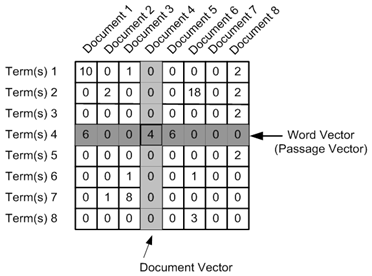
\includegraphics[width=0.4\textwidth]{images/matrix}
	\label{matrix}
\end{wrapfigure}

En esta sección, se calculará la matriz tf-idf (ver Figura~\ref{matrix}). Pero para ello, primero se tienen que calcular las frecuencias de las palabras que contienen los títulos, y el método más popular para hacerlo es el llamado \href{https://es.wikipedia.org/wiki/Tf-idf}{TF-IDF}. Este es un acrónimo que significa \textit{Frecuencia de Término – Frecuencia Inversa de Documento} que son los componentes de las puntuaciones resultantes asignadas a cada palabra. Sin entrar en la matemática, TF-IDF son puntuaciones de frecuencia de palabras que tratan de resaltar las palabras que son más interesantes y/o frecuentes. En el caso de la práctica usamos \href{https://scikit-learn.org/stable/modules/generated/sklearn.feature_extraction.text.TfidfVectorizer.html}{sklearn.feature\_extraction.text.TfidfVectorizer}.

\newpage 

\begin{lstlisting}[language=python]
tfidf_vectorizer = TfidfVectorizer(stop_words=stopwords, use_idf=True, 
	tokenizer=tokenize_and_stem, ngram_range=(1, 3))
									
# tokenize and build coded vocabulary
tfidf_matrix = tfidf_vectorizer.fit_transform(titles)
print(tfidf_matrix.shape)
>> (998, 7258)
\end{lstlisting}

La matriz tf-idf está formada por 998 términos y 7258 documentos. También se puede observar el vocabulario (nombrado \textit{terms}) que ha usado \textit{TfidfVectorizer} en la construcción de la matriz:

\begin{lstlisting}[language=python]
terms = tfidf_vectorizer.get_feature_names()
print(terms[:20])    # first 20 terms
>> ["'d", "'d go", "'d go bernadett", "'m", "'m gone", "'m home", "'m lie", "'m lie tell", "'s", "'s alic", "'s alic wonderland", "'s astound", "'s astound stori", "'s autobiographi", "'s babi", "'s babi ice", "'s berlin", "'s call", "'s call cormoran", "'s childhood"]
\end{lstlisting}

\begin{definition}\label{n_grama}
Un n-grama es una secuencia contigua de n elementos de una muestra determinada de texto o de un discurso. Los elementos pueden ser fonemas, sílabas, letras o palabras según la aplicación. Los n-gramas normalmente se recopilan de un texto.
\end{definition}

Un par de cosas a tener en cuenta sobre los parámetros definidos en la función \textit{TfidfVectorizer}:

\begin{itemize}
	\item use\_idf: habilita la reponderación de frecuencia de documentos inversa.
	\item ngram\_range: define el límite inferior y superior del rango de n-valores para diferentes n-gramas que se extraerán. Ver Definición~\ref{n_grama}.
\end{itemize}

\subsection{Entrenamiento del algoritmo}

Ahora pasamos a la parte divertida. Usando la matriz tf-idf calculada en la sección anterior, se puede ejecutar el algoritmo K-Means utilizando \href{https://scikit-learn.org/stable/modules/generated/sklearn.cluster.KMeans.html}{sklearn.cluster.KMeans}, para comprender mejor la estructura oculta dentro de los títulos de los libros. El algoritmo K-Means se inicializa con un número predeterminado de clústeres. Elegí el número 40 como número predeterminado de clústeres, ya que el conjunto de datos de entrada contiene libros que pertenecen al menos a más de dos de las 50 categorías existentes en el conjunto de datos, descartando 10 categorías que solo hacen referencia a un único libro.

\begin{lstlisting}[language=python]
num_clusters = 40
km = KMeans(n_clusters=num_clusters)
km.fit(tfidf_matrix)
clusters = km.labels_.tolist()
\end{lstlisting}

Para analizar los resultados y visualizar los clústeres (\textit{clusters}), ha sido necesario crear dos nuevos dataframes. Uno que contenga los títulos y sus clústeres asignados (\textit{frame}), y otro que contenga las raíces de los títulos con sus palabras asignadas (\textit{vocab\_frame}). Para crear el segundo, además, ha sido necesario crear dos nuevos vocabularios: uno que contenga los títulos tokanizados y otro que contenga las raíces de los títulos tokanizados. Para ello se han usado las funciones: \textit{tokenize\_and\_stem} y \textit{tokenize\_only}, ya nombradas anteriormente (ver Sección~\ref{stem_token}).

\begin{lstlisting}[language=python]
# new df with titles and clusters
frame = pd.DataFrame({'title': titles, 'cluster': clusters}, index=[clusters], 
	columns=['title', 'cluster'])
\end{lstlisting}

\newpage
\begin{lstlisting}[language=python]
# new two vocabularies: stemmed and tokenized
totalvocab_stemmed = []
totalvocab_tokenized = []
for i in titles:
	allwords_stemmed = tokenize_and_stem(i)  # for each item in 'titles', tokenize/stem
	totalvocab_stemmed.extend(allwords_stemmed)  # extend the 'totalvocab_stemmed' list

	allwords_tokenized = tokenize_only(i)
	totalvocab_tokenized.extend(allwords_tokenized)
	
vocab_frame = pd.DataFrame({'words': totalvocab_tokenized}, index=totalvocab_stemmed)
print('There are ' + str(vocab_frame.shape[0]) + ' items in vocab_frame')
>> There are 6371 items in vocab_frame
\end{lstlisting}

El beneficio de este procedimiento es que proporciona una forma eficiente de buscar una raíz y devolver la palabra que la contiene muy rápidamente. La desventaja es que hay demasiadas raíces, concretamente 6371. Por ejemplo, la raíz 'run' podría estar asociada con 'ran', 'runs', 'running', etc. Aunque para mi propósito de visualización de los clústeres está bien. A continuación podemos observar las primeras líneas del contenido de los dos nuevos dataframes.

\begin{table}[!htb]
	\centering
	\caption{\textit{frame} y \textit{vocab\_frame} dataframes.}
	\begin{minipage}{.6\linewidth}
		\centering
		\begin{tabular}{lc}
			\toprule
			title &  cluster \\
			\midrule
			Sapiens: A Brief History of Humankind & 26 \\
			Sharp Objects & 0 \\
			Soumission & 12 \\
			Tipping the Velvet & 12 \\
			A Light in the Attic & 9 \\
			\bottomrule
		\end{tabular}
	\end{minipage}%
	\begin{minipage}{.4\linewidth}
		\centering
		\begin{tabular}{lc}
			\toprule
			& words \\
			\midrule
			sapien & sapiens \\
			a & a \\
			brief & brief \\
			histori & history \\
			of & of \\
			\bottomrule
		\end{tabular}
	\end{minipage} 
\end{table}

Finalmente, vemos la función implementada que muestra los resultados por clúster, identificando las $n$ primeras palabras (elegí $n$=10) que están más cerca de los centroides de cada uno de ellos, y también vemos el resultado de su ejecución (ver Figura~\ref{results}). 

\begin{lstlisting}[language=python]
# sort cluster centers by proximity to centroid	
order_centroids = km.cluster_centers_.argsort()[:, ::-1] 

for i in range(num_clusters):
	print("Cluster {} words:".format(i), end='')
	for ind in order_centroids[i, :10]:  # replace 10 with n words per cluster
		print(' {}'.format(vocab_frame.loc[terms[ind].split(' ')].values.tolist()[0][0]), 
			end=',')
	
	print()
	print()
	
	print("Cluster {} titles:".format(i), end='')
	for title in frame.loc[i]['title'].values.tolist():
		print(' {},'.format(title), end='')
	
	print()
	print()
\end{lstlisting}

\begin{figure}
	\centering
	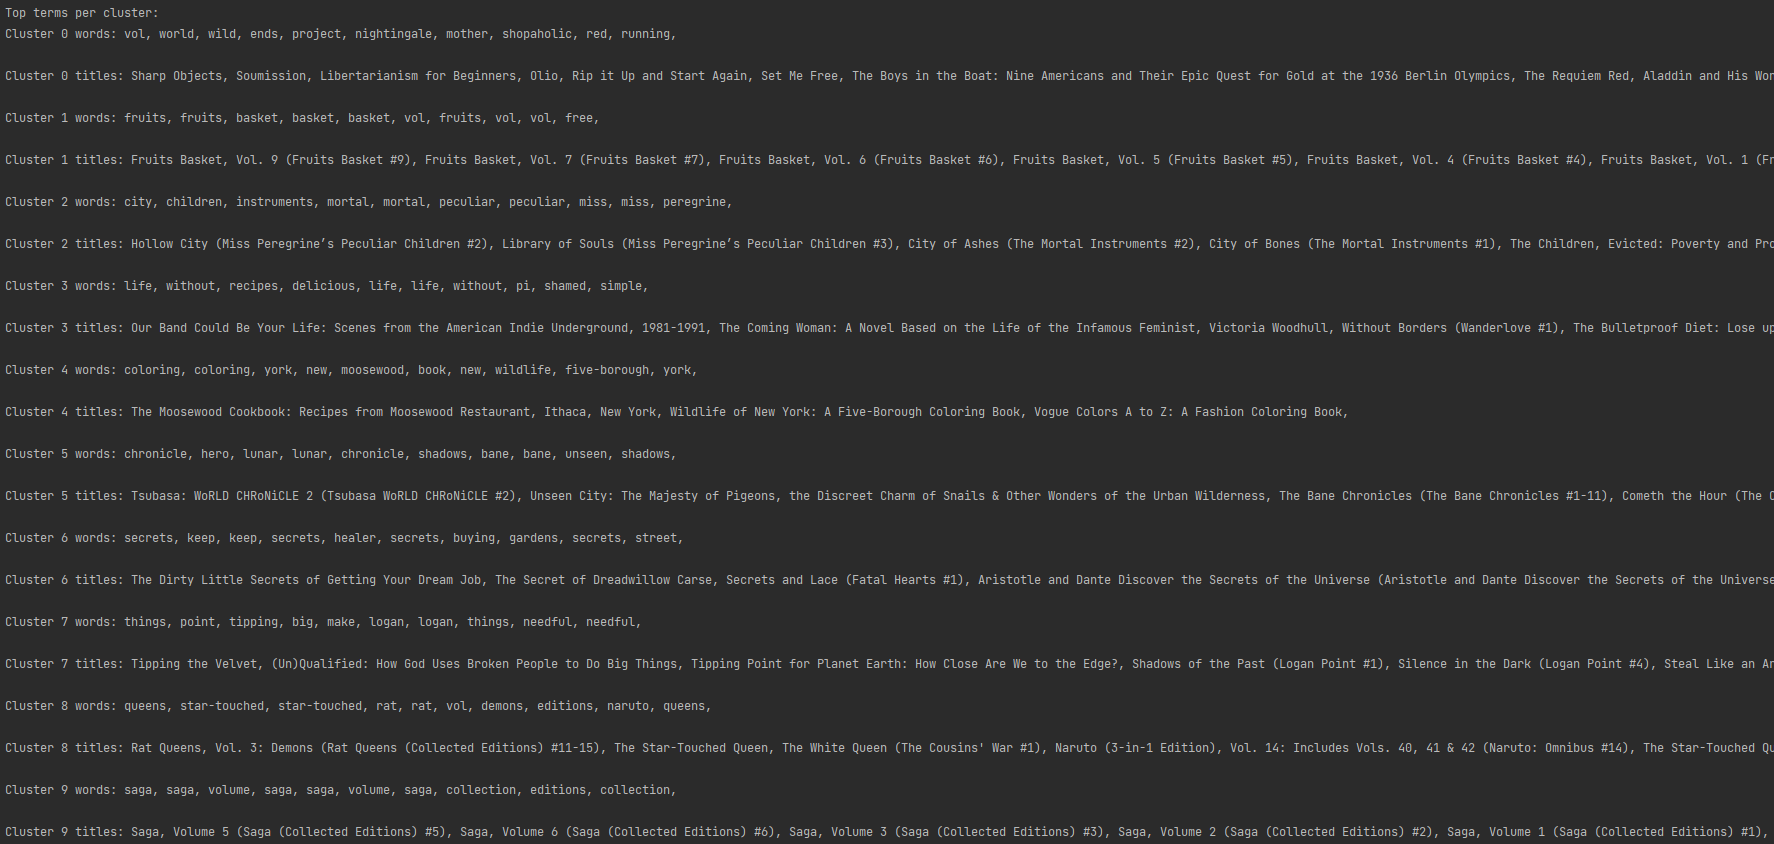
\includegraphics[scale=0.35]{images/results}
	\caption{Resultados del proceso de \textit{clustering}.}
	\label{results}
\end{figure}

\subsection{Evaluación}


\renewcommand{\refname}{Bibliografía}
\bibliographystyle{unsrt}
\bibliography{biblio}

\end{document}
